\section{Problem Description}\label{sec:prob_descr}
An unbalanced levered helicopter needs to be balanced using optimizing control.
The complete model of the helicopter is outlined in \Cref{eq:model}.
\begin{subequations}\label{eq:model}
	\begin{align}
		\ddot{e} + K_{3} K_{ed} \dot{e} + K_{3} K_{ep} e = K_{3} K_{ep} e_{c} \label{eq:model_se_elev} \\
		\ddot{p} + K_{1} K_{pd} \dot{p} + K_{1} K_{pp} p = K_{1} K_{pp} p_{c} \label{eq:model_se_pitch} \\
		\dot{\lambda} = r \label{eq:model_se_lambda} \\
		\dot{r} = -K_{2} p \label{eq:model_se_r}
	\end{align}
\end{subequations}

The specific exercises can be found in sections 10.2, 10.3, and 10.4 of \Cref{sec:ex}.

\Cref{fig:layers_openloop} shows the lab setup containing a lever. Its right side (from the viewer's perspective) contains a mass to balance the lever to some extent, and on the left side two motors serve as the helicopter. The motors are powered off in the picture, and is set up such that the direction of force from the blades goes against the force of gravity. The middle of the lever is connected to power and measuring devices such that its movement can be tracked.

\begin{figure}[tp]
\centering
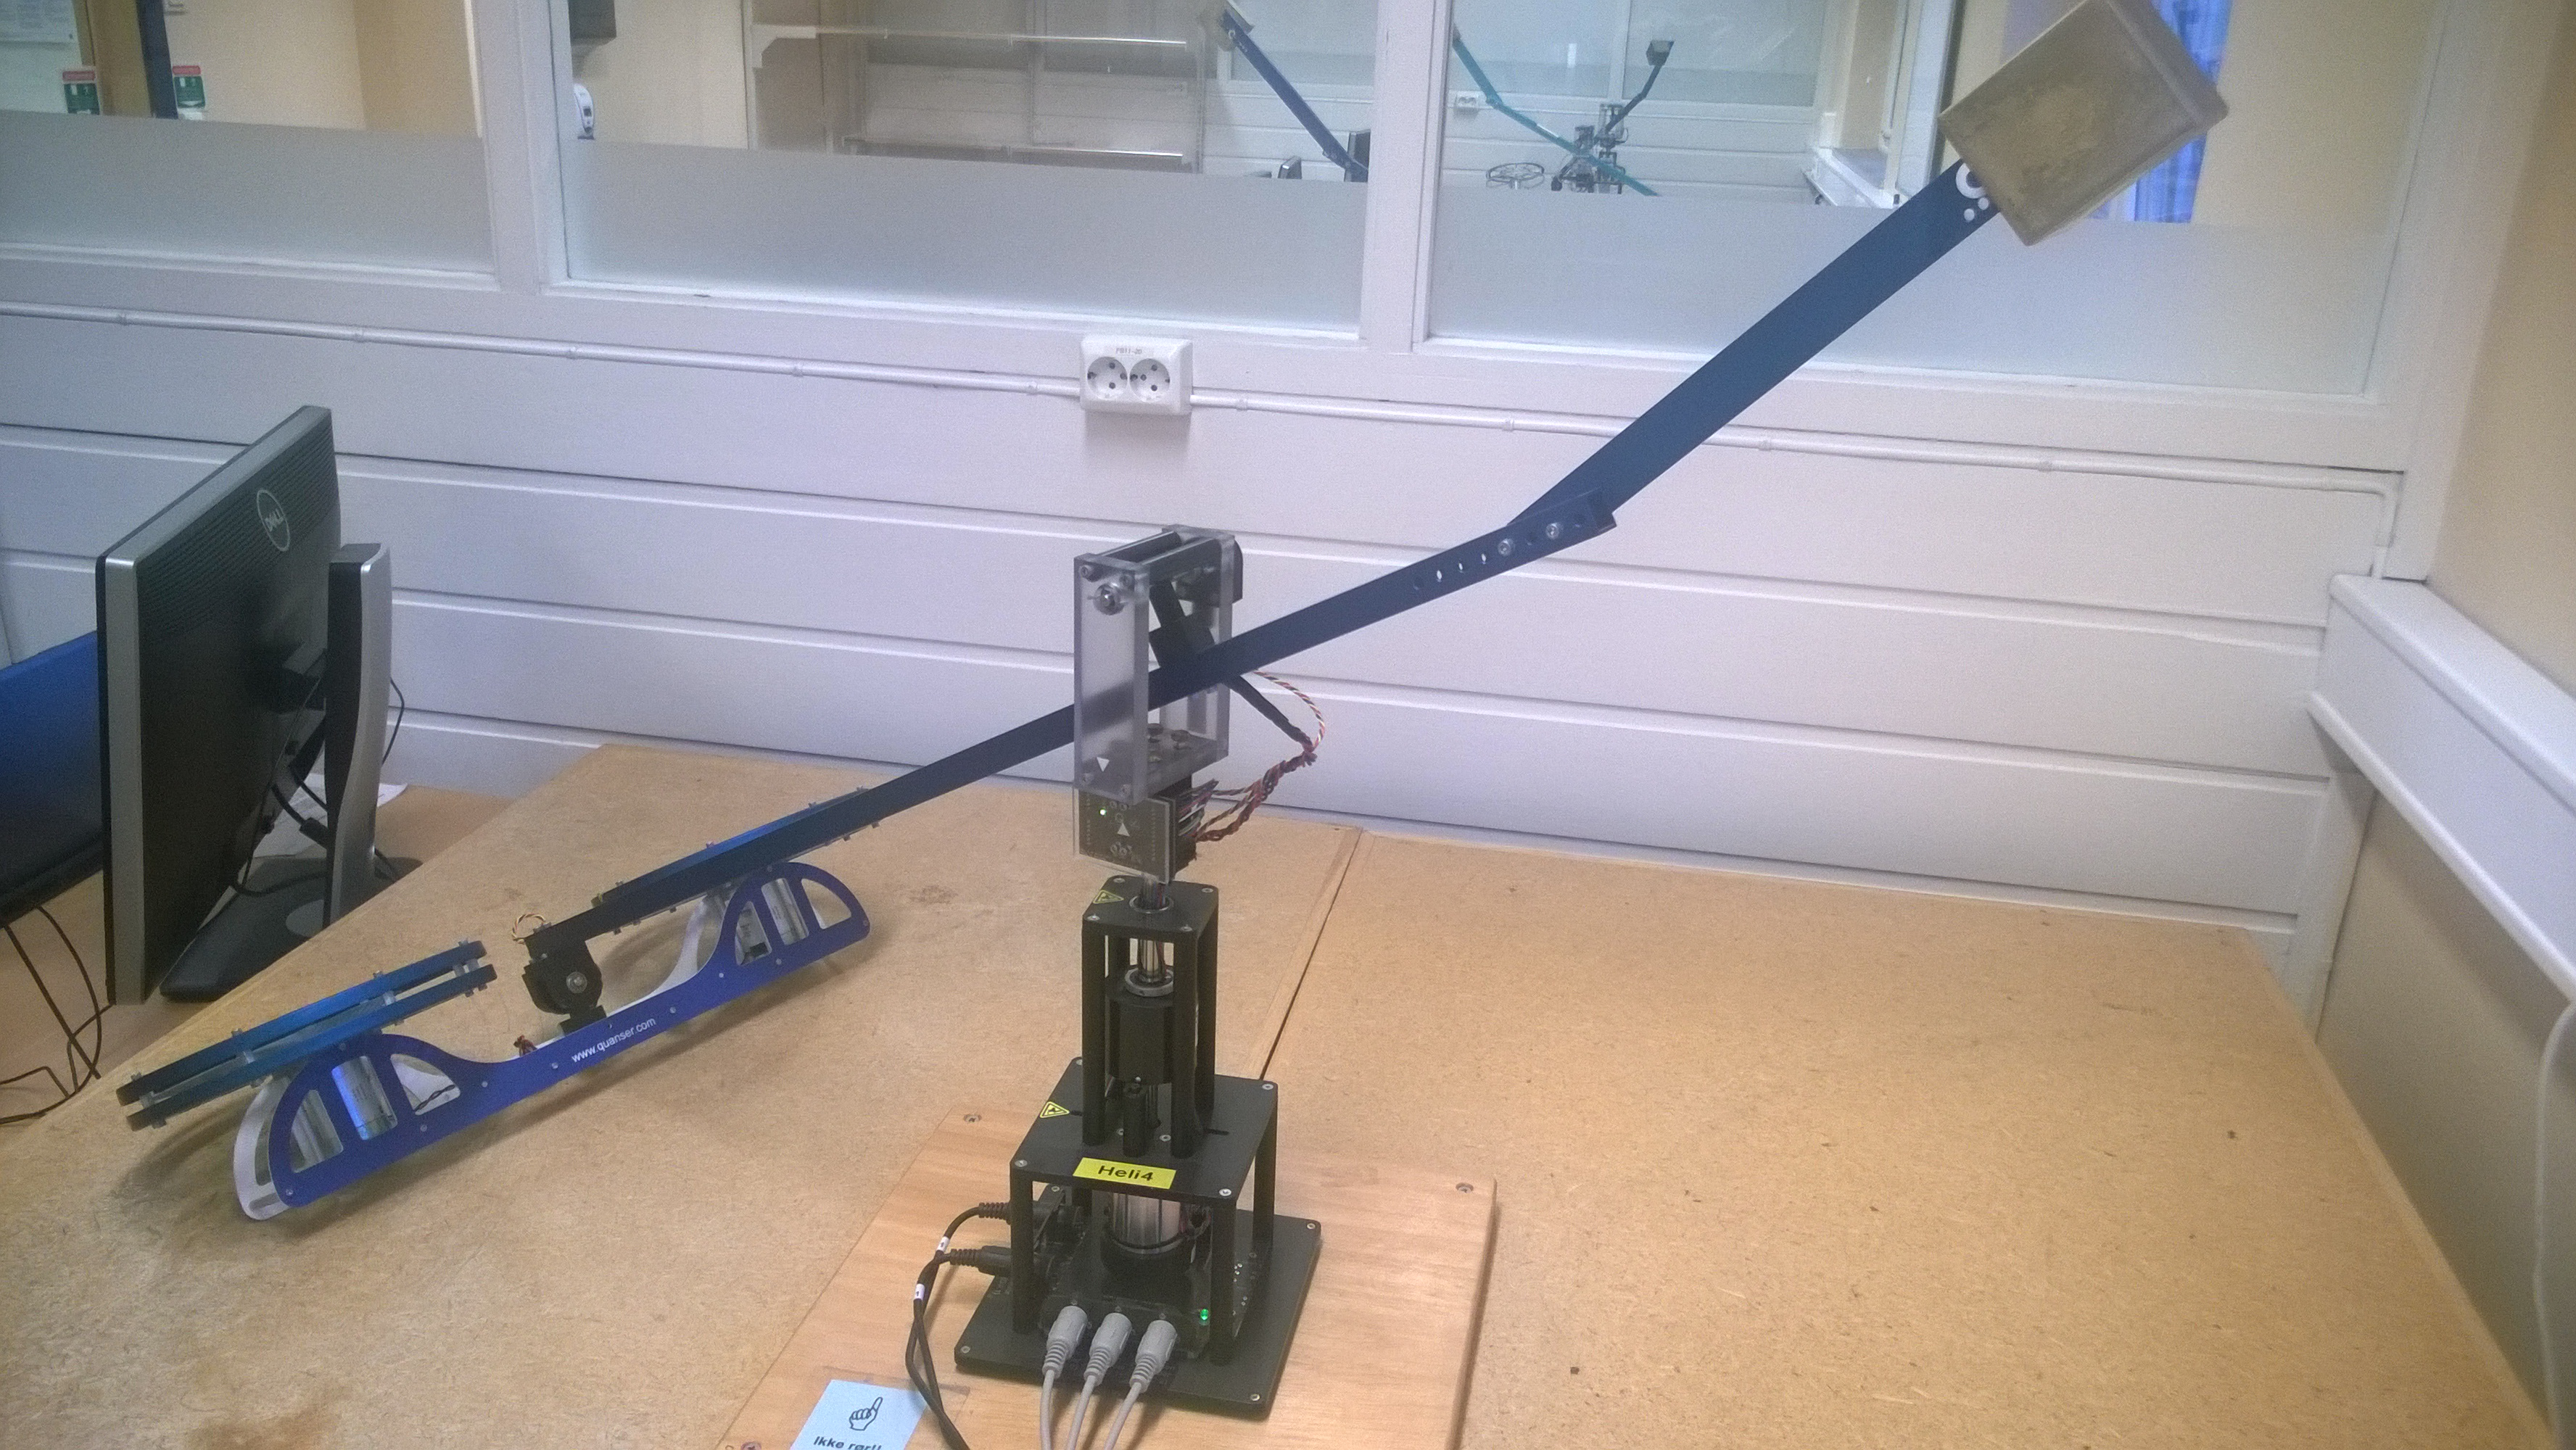
\includegraphics[width=1.00\textwidth]{figures/WP_20170426_003.jpg}
\caption{The levered helicopter as it is set up in the lab.}
\label{fig:layers_openloop}
\end{figure}
